\begin{figure}[H]
	\centering
	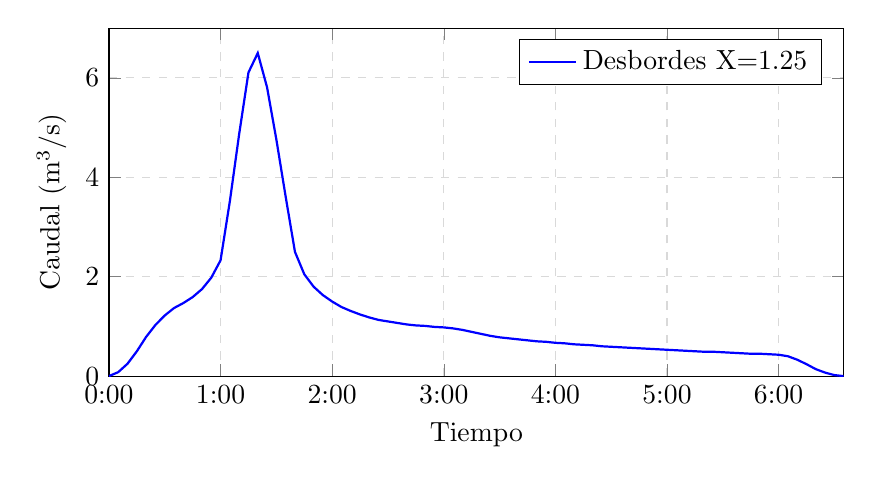
\begin{tikzpicture}
		\begin{axis}[
			width=0.9\textwidth,
			height=6cm,
			xlabel={Tiempo},
			ylabel={Caudal (m$^3$/s)},
			xmin=0,
			xmax=395,
			ymin=0,
			ymax=7,
			grid=major,
			grid style={dashed, gray!30},
			legend pos=north east,
			xtick={0, 60, 120, 180, 240, 300, 360},
			xticklabels={0:00, 1:00, 2:00, 3:00, 4:00, 5:00, 6:00},
			]
		% Desbordes X=1.25
		\addplot [
		blue,
		thick,
		solid,
		] coordinates {
				(0, 0.00) (5, 0.08) (10, 0.25) (15, 0.50) (20, 0.79)
				(25, 1.03) (30, 1.22) (35, 1.37) (40, 1.47) (45, 1.59)
				(50, 1.75) (55, 1.98) (60, 2.33) (65, 3.52) (70, 4.87)
				(75, 6.11) (80, 6.50) (85, 5.81) (90, 4.76) (95, 3.61)
				(100, 2.50) (105, 2.05) (110, 1.80) (115, 1.63) (120, 1.50)
				(125, 1.39) (130, 1.31) (135, 1.24) (140, 1.18) (145, 1.13)
				(150, 1.10) (155, 1.07) (160, 1.04) (165, 1.02) (170, 1.01)
				(175, 0.99) (180, 0.98) (185, 0.96) (190, 0.93) (195, 0.89)
				(200, 0.85) (205, 0.81) (210, 0.78) (215, 0.76) (220, 0.74)
				(225, 0.72) (230, 0.70) (235, 0.69) (240, 0.67) (245, 0.66)
				(250, 0.64) (255, 0.63) (260, 0.62) (265, 0.60) (270, 0.59)
				(275, 0.58) (280, 0.57) (285, 0.56) (290, 0.55) (295, 0.54)
				(300, 0.53) (305, 0.52) (310, 0.51) (315, 0.50) (320, 0.49)
				(325, 0.49) (330, 0.48) (335, 0.47) (340, 0.46) (345, 0.45)
				(350, 0.45) (355, 0.44) (360, 0.43) (365, 0.40) (370, 0.33)
				(375, 0.24) (380, 0.14) (385, 0.07) (390, 0.02) (395, 0.00)
		};
		\addlegendentry{Desbordes X=1.25}

		\end{axis}
	\end{tikzpicture}
	\caption{Hidrograma - Desbordes + GZ $T_r$=2 años ($Q_p$=6.503 m$^3$/s)}
	\label{fig:hydro_desbordes_gz_Tr2_X125}
\end{figure}
